\documentclass[aspectratio=1610, 10pt, notheorems]{beamer}
\usetheme{Warsaw} 
\usecolortheme{seahorse}

%%% Кодировка и локализация %%%
\usepackage[utf8]{inputenc} % кодовая страница документа
\usepackage[T2A]{fontenc} % внутренняя кодировка  TeX
\usepackage[english,russian]{babel} % локализация и переносы

%%% Гипперссылки и pdf %%%
\usepackage{cmap} % русский поиск в pdf
\usepackage{hyperref} % гиперссылки

%%% Пакеты для формул %%%
\usepackage{amsmath} % удобная вёрстка многострочных формул, масштабирующийся текст в формулах, формулы в рамках и др.
\usepackage{amssymb} % несколько сотен дополнительных математических символов
\usepackage{amsthm} % окружения «теорема», «лемма» и т. п.
\usepackage{amsfonts} % Ажурный \mathbb{} и готический \mathfrak{} шрифты
\usepackage{mathrsfs} % Mathematical Script letters (шрифт Эйлера) \mathscr{}
\usepackage{euscript} % Шрифт Евклида \EuScript{}
% каллиграфический шрифт \mathcal{} не требует пакета
\usepackage{enumitem}
\usepackage{bm}
\usepackage{multicol}

%%% Графика, изображения и цвета %%%
\usepackage{graphicx} % Работа с графикой \includegraphics{}
\usepackage{float} % Фиксация плавабщих боксов [H]
\graphicspath{
    {./images/}, 
    {./images/img1/}, 
    {./images/img2/}, 
    {./images/img3/}, 
    {./images/tikz1/}, 
    {./images/tikz2/}, 
    {./images/tikz3/},
    {./images/tree/},
    {./images/presentation/},
    }
    
\newtheorem{theorem}     {Теорема}
\newtheorem{lemma}       {Лемма}
\newtheorem{proposition} {Предложение}
\newtheorem{corollary}   {Следствие}
\newtheorem{definition}  {Определение}
\newtheorem{example}     {Пример} 
\newtheorem{remark}      {Замечание}
   
%%% Настройки презентации %%%
\everymath{\color{blue}}    % цвет формул в текстмоде
\everydisplay{\color{blue}} % цвет выключных формул
\setbeamertemplate{navigation symbols}{} % Убрать панель навигации
% \setbeamertemplate{footline}[frame number] % Номера слайдов вместо нижней строки
\setbeamertemplate{page number in head/foot}[totalframenumber]
\setbeamertemplate{bibliography item}{\insertbiblabel}
\hypersetup{unicode=true} % разрешить использование символов Юникод в закладках. настройка для hiperref

%%% Русская традиция начертания математических знаков
\renewcommand{\le}  {\ensuremath{\leqslant}}
\renewcommand{\leq} {\ensuremath{\leqslant}}
\renewcommand{\ge}  {\ensuremath{\geqslant}}
\renewcommand{\geq} {\ensuremath{\geqslant}}
\renewcommand{\emptyset}{\varnothing}

%%% Русская традиция начертания математических функций (на случай копирования из зарубежных источников)
\renewcommand{\tan}{\operatorname{tg}}
\renewcommand{\cot}{\operatorname{ctg}}
\renewcommand{\csc}{\operatorname{cosec}}

%%% Русская традиция начертания греческих букв (греческие буквы вертикальные, через пакет upgreek)
% \usepackage{upgreek} % прямые греческие ради русской традиции
% \renewcommand{\epsilon}{\ensuremath{\upvarepsilon}}   %  русская традиция записи
% \renewcommand{\phi}{\ensuremath{\upvarphi}}
% %\renewcommand{\kappa}{\ensuremath{\varkappa}}
% \renewcommand{\alpha}{\upalpha}
% \renewcommand{\beta}{\upbeta}
% \renewcommand{\gamma}{\upgamma}
% \renewcommand{\delta}{\updelta}
% \renewcommand{\varepsilon}{\upvarepsilon}
% \renewcommand{\zeta}{\upzeta}
% \renewcommand{\eta}{\upeta}
% \renewcommand{\theta}{\uptheta}
% \renewcommand{\vartheta}{\upvartheta}
% \renewcommand{\iota}{\upiota}
% \renewcommand{\kappa}{\upkappa}
% \renewcommand{\lambda}{\uplambda}
% \renewcommand{\mu}{\upmu}
% \renewcommand{\nu}{\upnu}
% \renewcommand{\xi}{\upxi}
% \renewcommand{\pi}{\uppi}
% \renewcommand{\varpi}{\upvarpi}
% \renewcommand{\rho}{\uprho}
% %\renewcommand{\varrho}{\upvarrho}
% \renewcommand{\sigma}{\upsigma}
% %\renewcommand{\varsigma}{\upvarsigma}
% \renewcommand{\tau}{\uptau}
% \renewcommand{\upsilon}{\upupsilon}
% \renewcommand{\varphi}{\upvarphi}
% \renewcommand{\chi}{\upchi}
% \renewcommand{\psi}{\uppsi}
% \renewcommand{\omega}{\upomega}



\newcommand {\rr}  {\mathbb{R}}
\newcommand {\nn}  {\mathbb{N}}
\newcommand {\zz}  {\mathbb{Z}}
\newcommand {\bbc} {\mathbb{C}}
% \newcommand {\rd}  {\mathbb{R}^d}
% \newcommand {\rpo} {\mathbb{R}_+^1}

\newcommand {\al} {\alpha}
\newcommand {\be} {\beta}
\newcommand {\da} {\delta}
\newcommand {\Da} {\Delta}
\newcommand {\Dl} {\Delta}
\newcommand {\ga} {\gamma}
\newcommand {\Ga} {\Gamma}
\newcommand {\la} {\lambda}
\newcommand {\La} {\Lambda}
\newcommand {\om} {\omega}
\newcommand {\Om} {\Omega}
\newcommand {\sa} {\sigma}
\newcommand {\Sa} {\Sigma}
\newcommand {\te} {\theta}
\newcommand {\fy} {\varphi}
\newcommand {\Fy} {\varPhi}
\newcommand {\ep} {\varepsilon}
\newcommand {\ro} {\varrho}

\newcommand{\bd}{{\bm{d}}}
\newcommand{\bj}{{\bm{j}}}
\newcommand{\bi}{{\bm{i}}}
\newcommand{\bk}{{\bm{k}}}
\newcommand{\bu}{{\bm{u}}}
\newcommand{\bx}{{\bm{x}}}
\newcommand{\bl}{{\bf{l}}}
\newcommand{\bma}{{\bm{\alpha}}}
\newcommand{\bmb}{{\bm{\beta}}}
\newcommand{\bmg}{{\bm{\gamma}}}

\newcommand {\ra}  {\rightarrow}
\newcommand {\IN}  {\subset}
\newcommand {\NI}  {\supset}
\newcommand {\mmm} {\setminus}
\newcommand {\8}   {\infty}
\newcommand {\io}  {I^\infty}
\newcommand {\ia}  {I^*}
\newcommand {\0}   {\varnothing}
\newcommand {\dd}  {\partial}
\newcommand {\pr}  {\mathrm{pr}}
% \renewcommand{\span}{\mathrm{span}}


\newcommand {\eA} {{\EuScript A}}
\newcommand {\eJ} {{\EuScript J}}
\newcommand {\eC} {{\EuScript C}}
\newcommand {\eU} {{\EuScript U}}
\newcommand {\eP} {{\EuScript P}}
\newcommand {\eS} {{\EuScript S}}
\newcommand {\eW} {{\EuScript W}}
\newcommand {\eZ} {{\EuScript Z}}
\newcommand {\eK} {{\EuScript K}}
\newcommand {\hT} {{\hat T}}
\newcommand {\wP} {{\widetilde P}}
\newcommand {\eV} {{\mathcal V}}

\def \diam {\mathop{\rm diam} \nolimits}
\def \sup  {\mathop{\rm sup}  \nolimits}
\def \fix  {\mathop{\rm fix}  \nolimits}
\def \Lip  {\mathop{\rm Lip}  \nolimits}
\def \min  {\mathop{\rm min}  \nolimits}
\def \Ln   {\mathop{\rm Ln}   \nolimits}
\def \Id   {\mathop{\rm Id}   \nolimits}

\newcommand{\red}{\textcolor{red}}     % Новые переменные и переименования

%%% Данные для титульного листа %%%
\title[Анализ на самоподобных множествах с конечным пересечением]
    {Анализ на самоподобных множествах с конечным пересечением}
\author[Dmitry Drozdov]
    {Дмитрий Дроздов \\ {\tt d.drozdov1@g.nsu.ru}}
\institute[ИМ СО РАН]{Институт математики имени С. Л. Соболева СО РАН}
\date[20.02.2024]
    {Семинар <<Геометрия, топология и их приложения>>\\10.06.2024}


\begin{document}


\begin{frame}{}
    \titlepage
\end{frame}


\section{Деформации полигональных дендритов}

\begin{frame}{Самоподобное множество}

\end{frame}


\begin{frame}{Дендрит}

\end{frame}


\begin{frame}{Стягиваемые $P$-полигональные  системы}
Даны многоугольник $P\IN \mathbb R^2$, множество его вершин $V_P=\{A_1,...,A_{n_P}\}$  и такая система подобий $\eS = \{S_1, \ldots, S_m\}$ в $\mathbb R^2$, что:\\
\only<1>{\[ 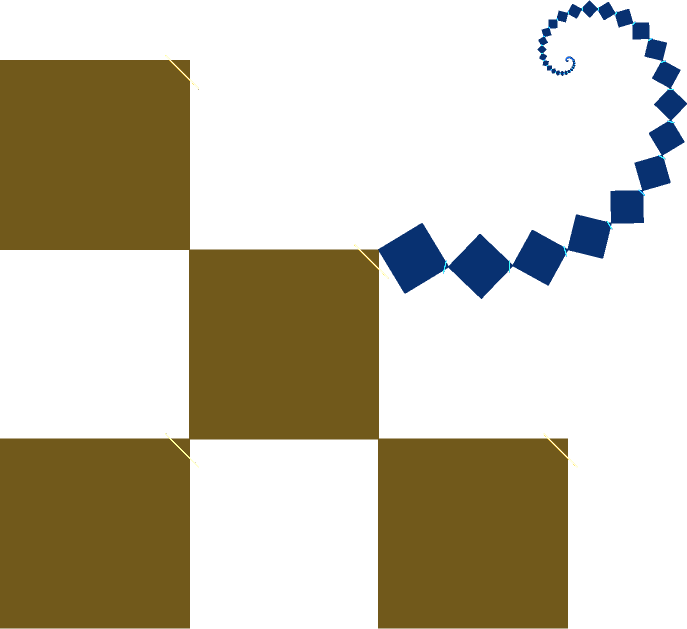
\includegraphics[width=.7\textwidth]{2_11.png}\]}
\only<2>{
{\bf(D1)}  для любого $i\in I$, множество $P_i=S_i(P)\IN P$;\\
\[ 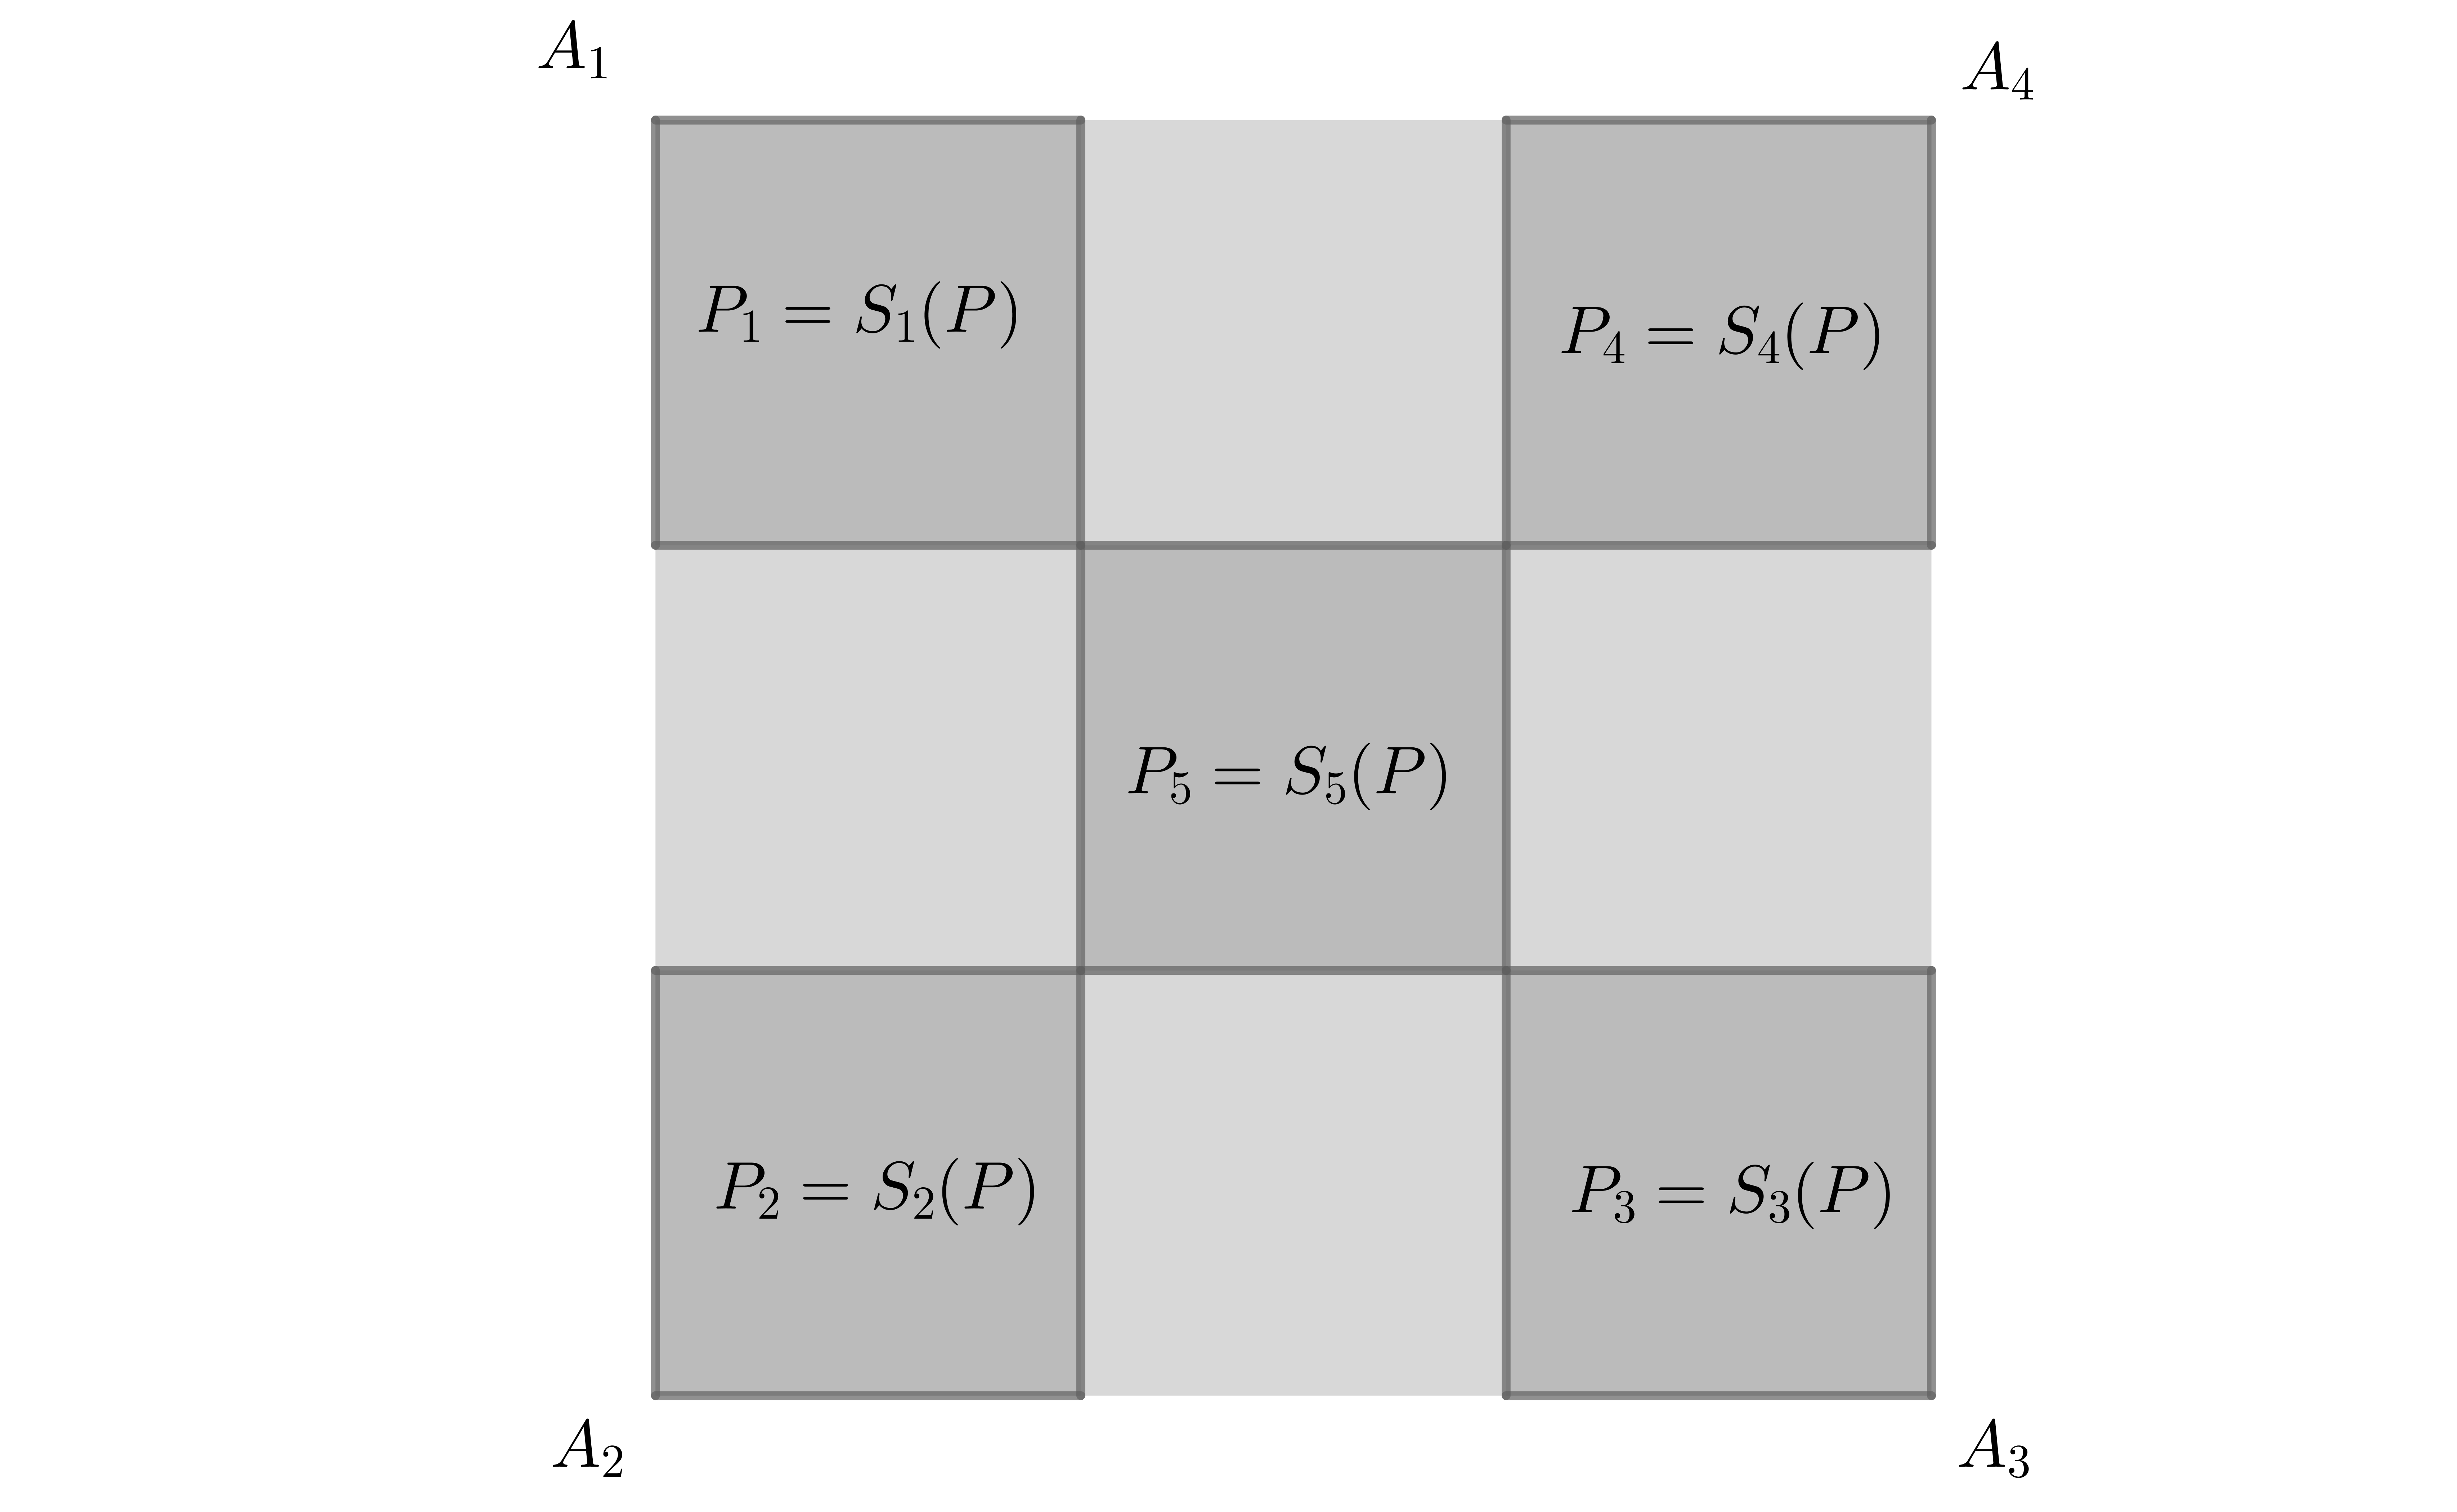
\includegraphics[width=.7\textwidth]{2_22.png}\]}
\only<3>{
{\bf(D1)}  для любого $i\in I$, множество $P_i=S_i(P)\IN P$;\\
{\bf(D2)}  для любых $i\neq j,\ \   i, j \in I,$ $P_i \cap P_j=V_{P_i}\cap V_{P_j}$ ;\\
\[ 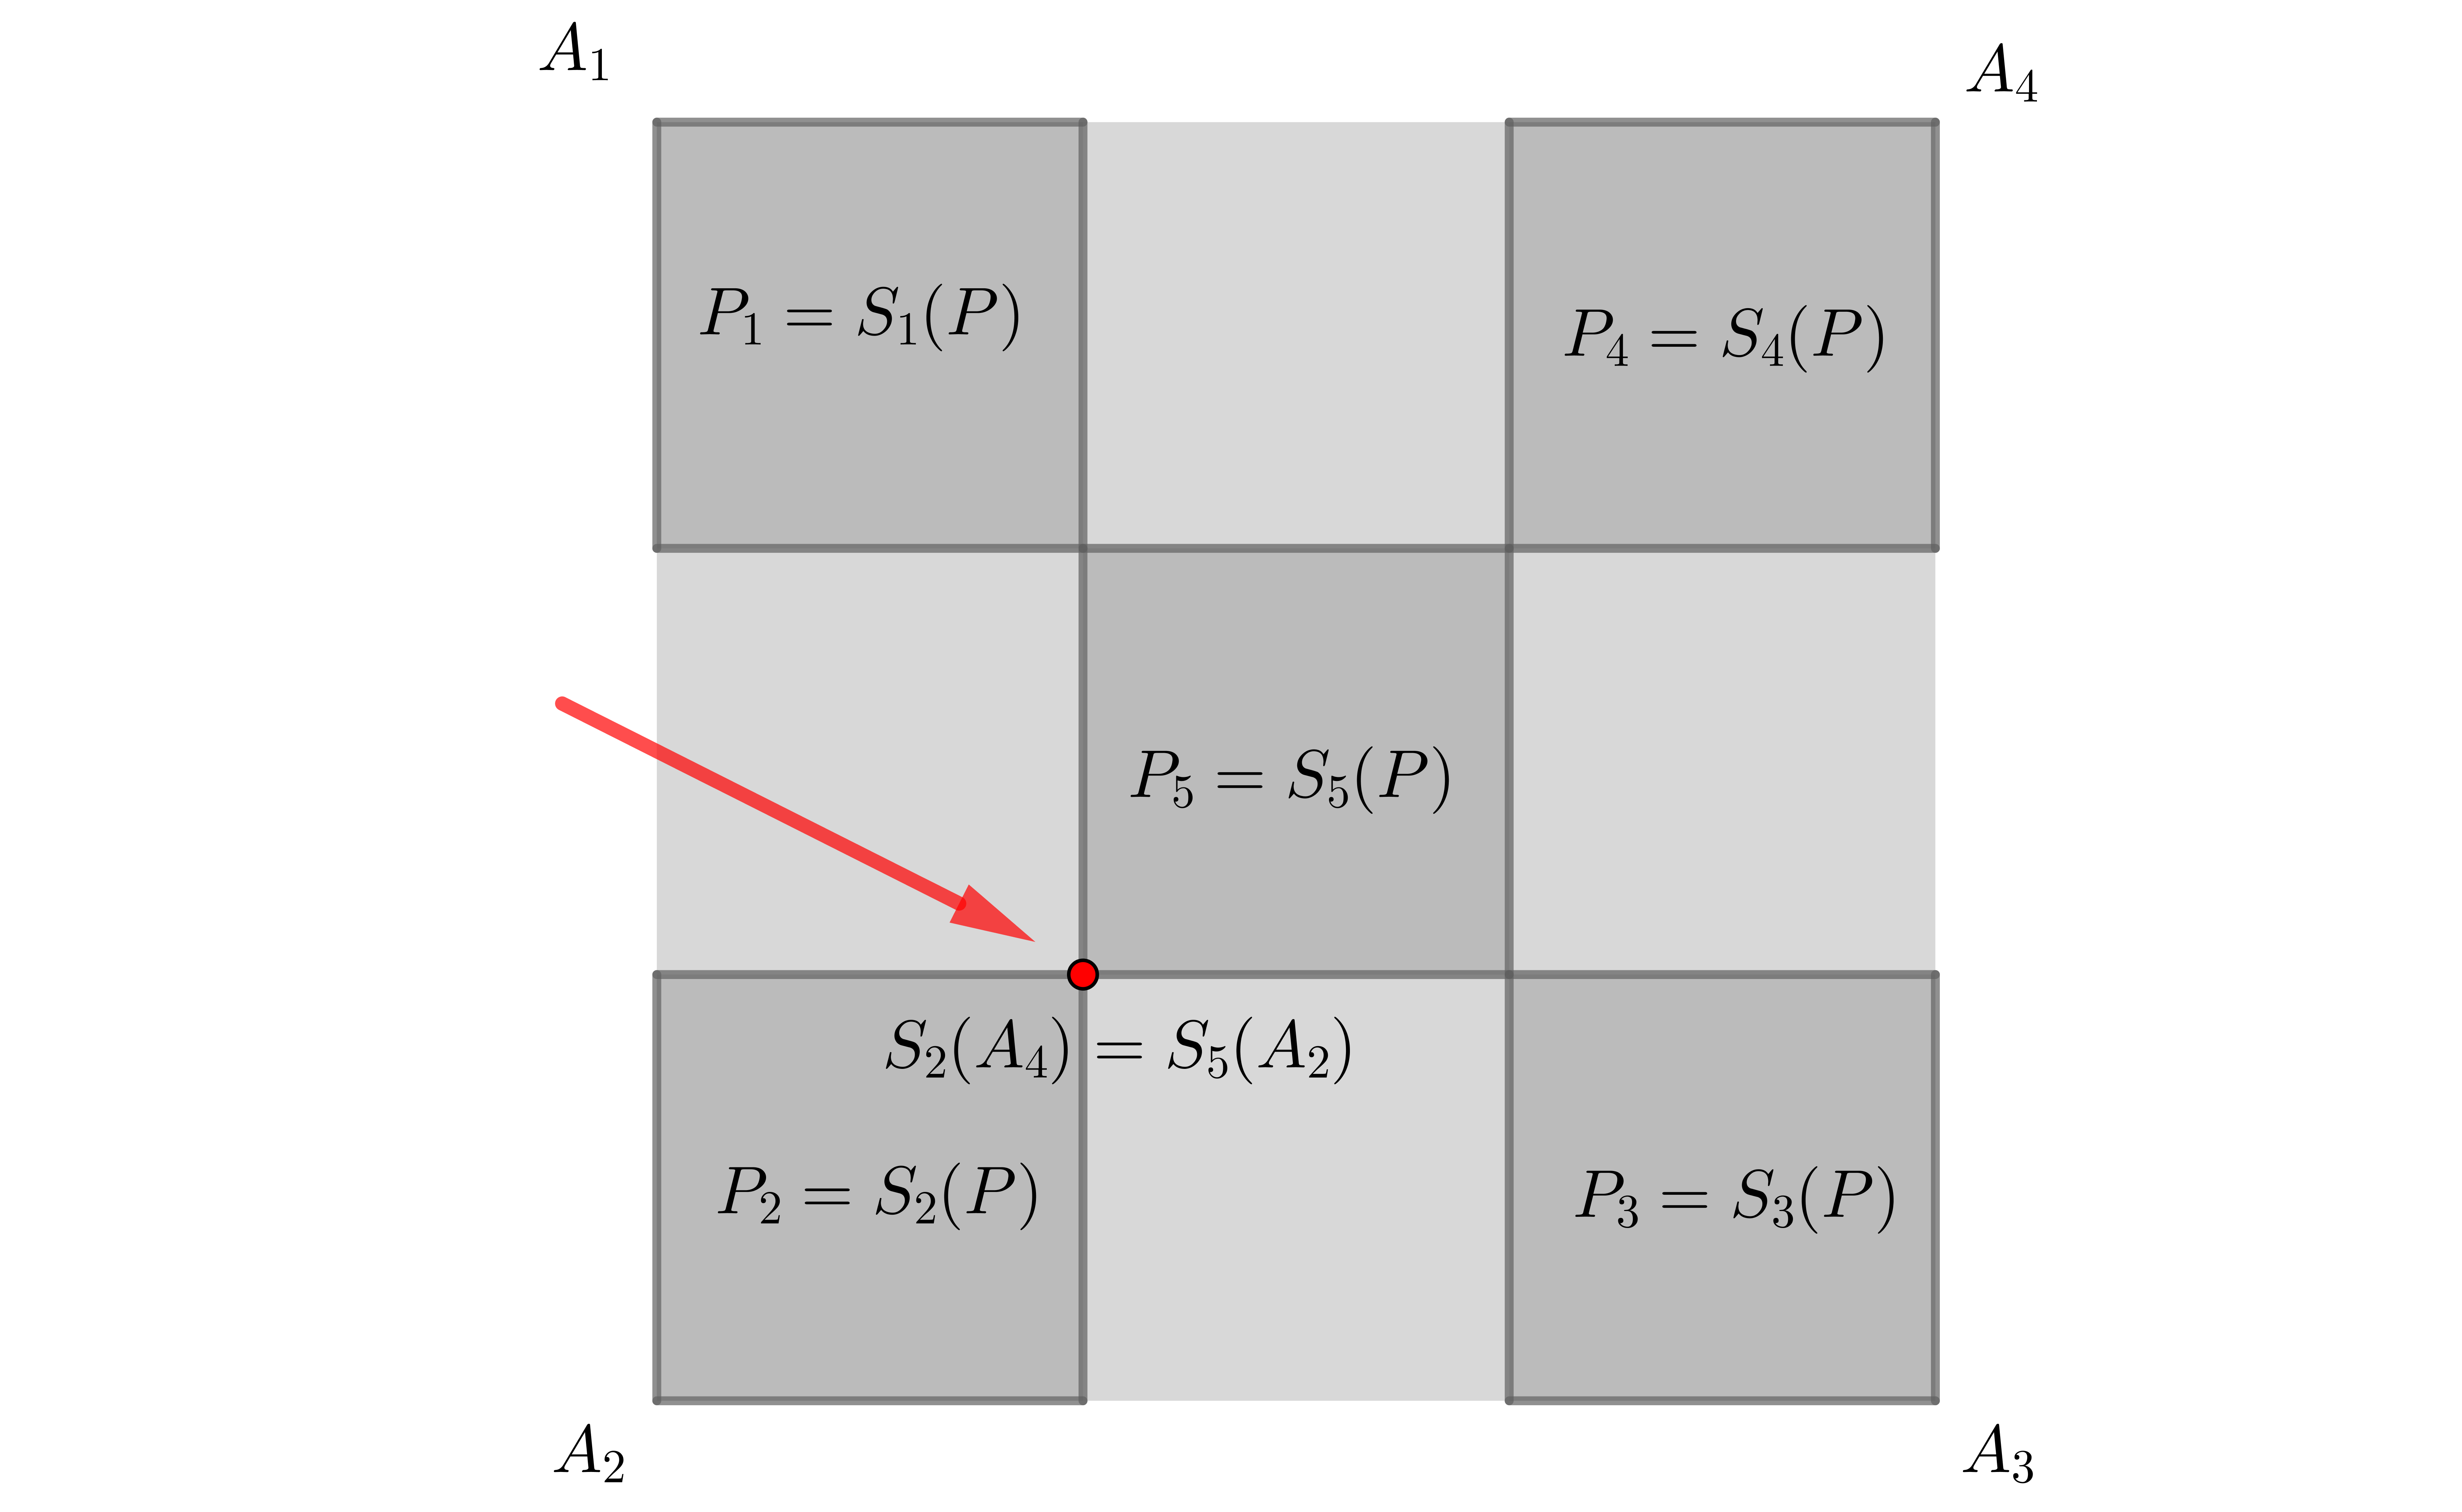
\includegraphics[width=.7\textwidth]{2_23.png}\]}
\only<4>{
{\bf(D1)}  для любого $i\in I$, множество $P_i=S_i(P)\IN P$;\\
{\bf(D2)}  для любых $i\neq j,\ \   i, j \in I,$ $P_i \cap P_j=V_{P_i}\cap V_{P_j}$ ;\\
{\bf(D3)}  $V_P\IN \bigcup\limits_{i\in I}S_i(V_P)$;\\
\[ 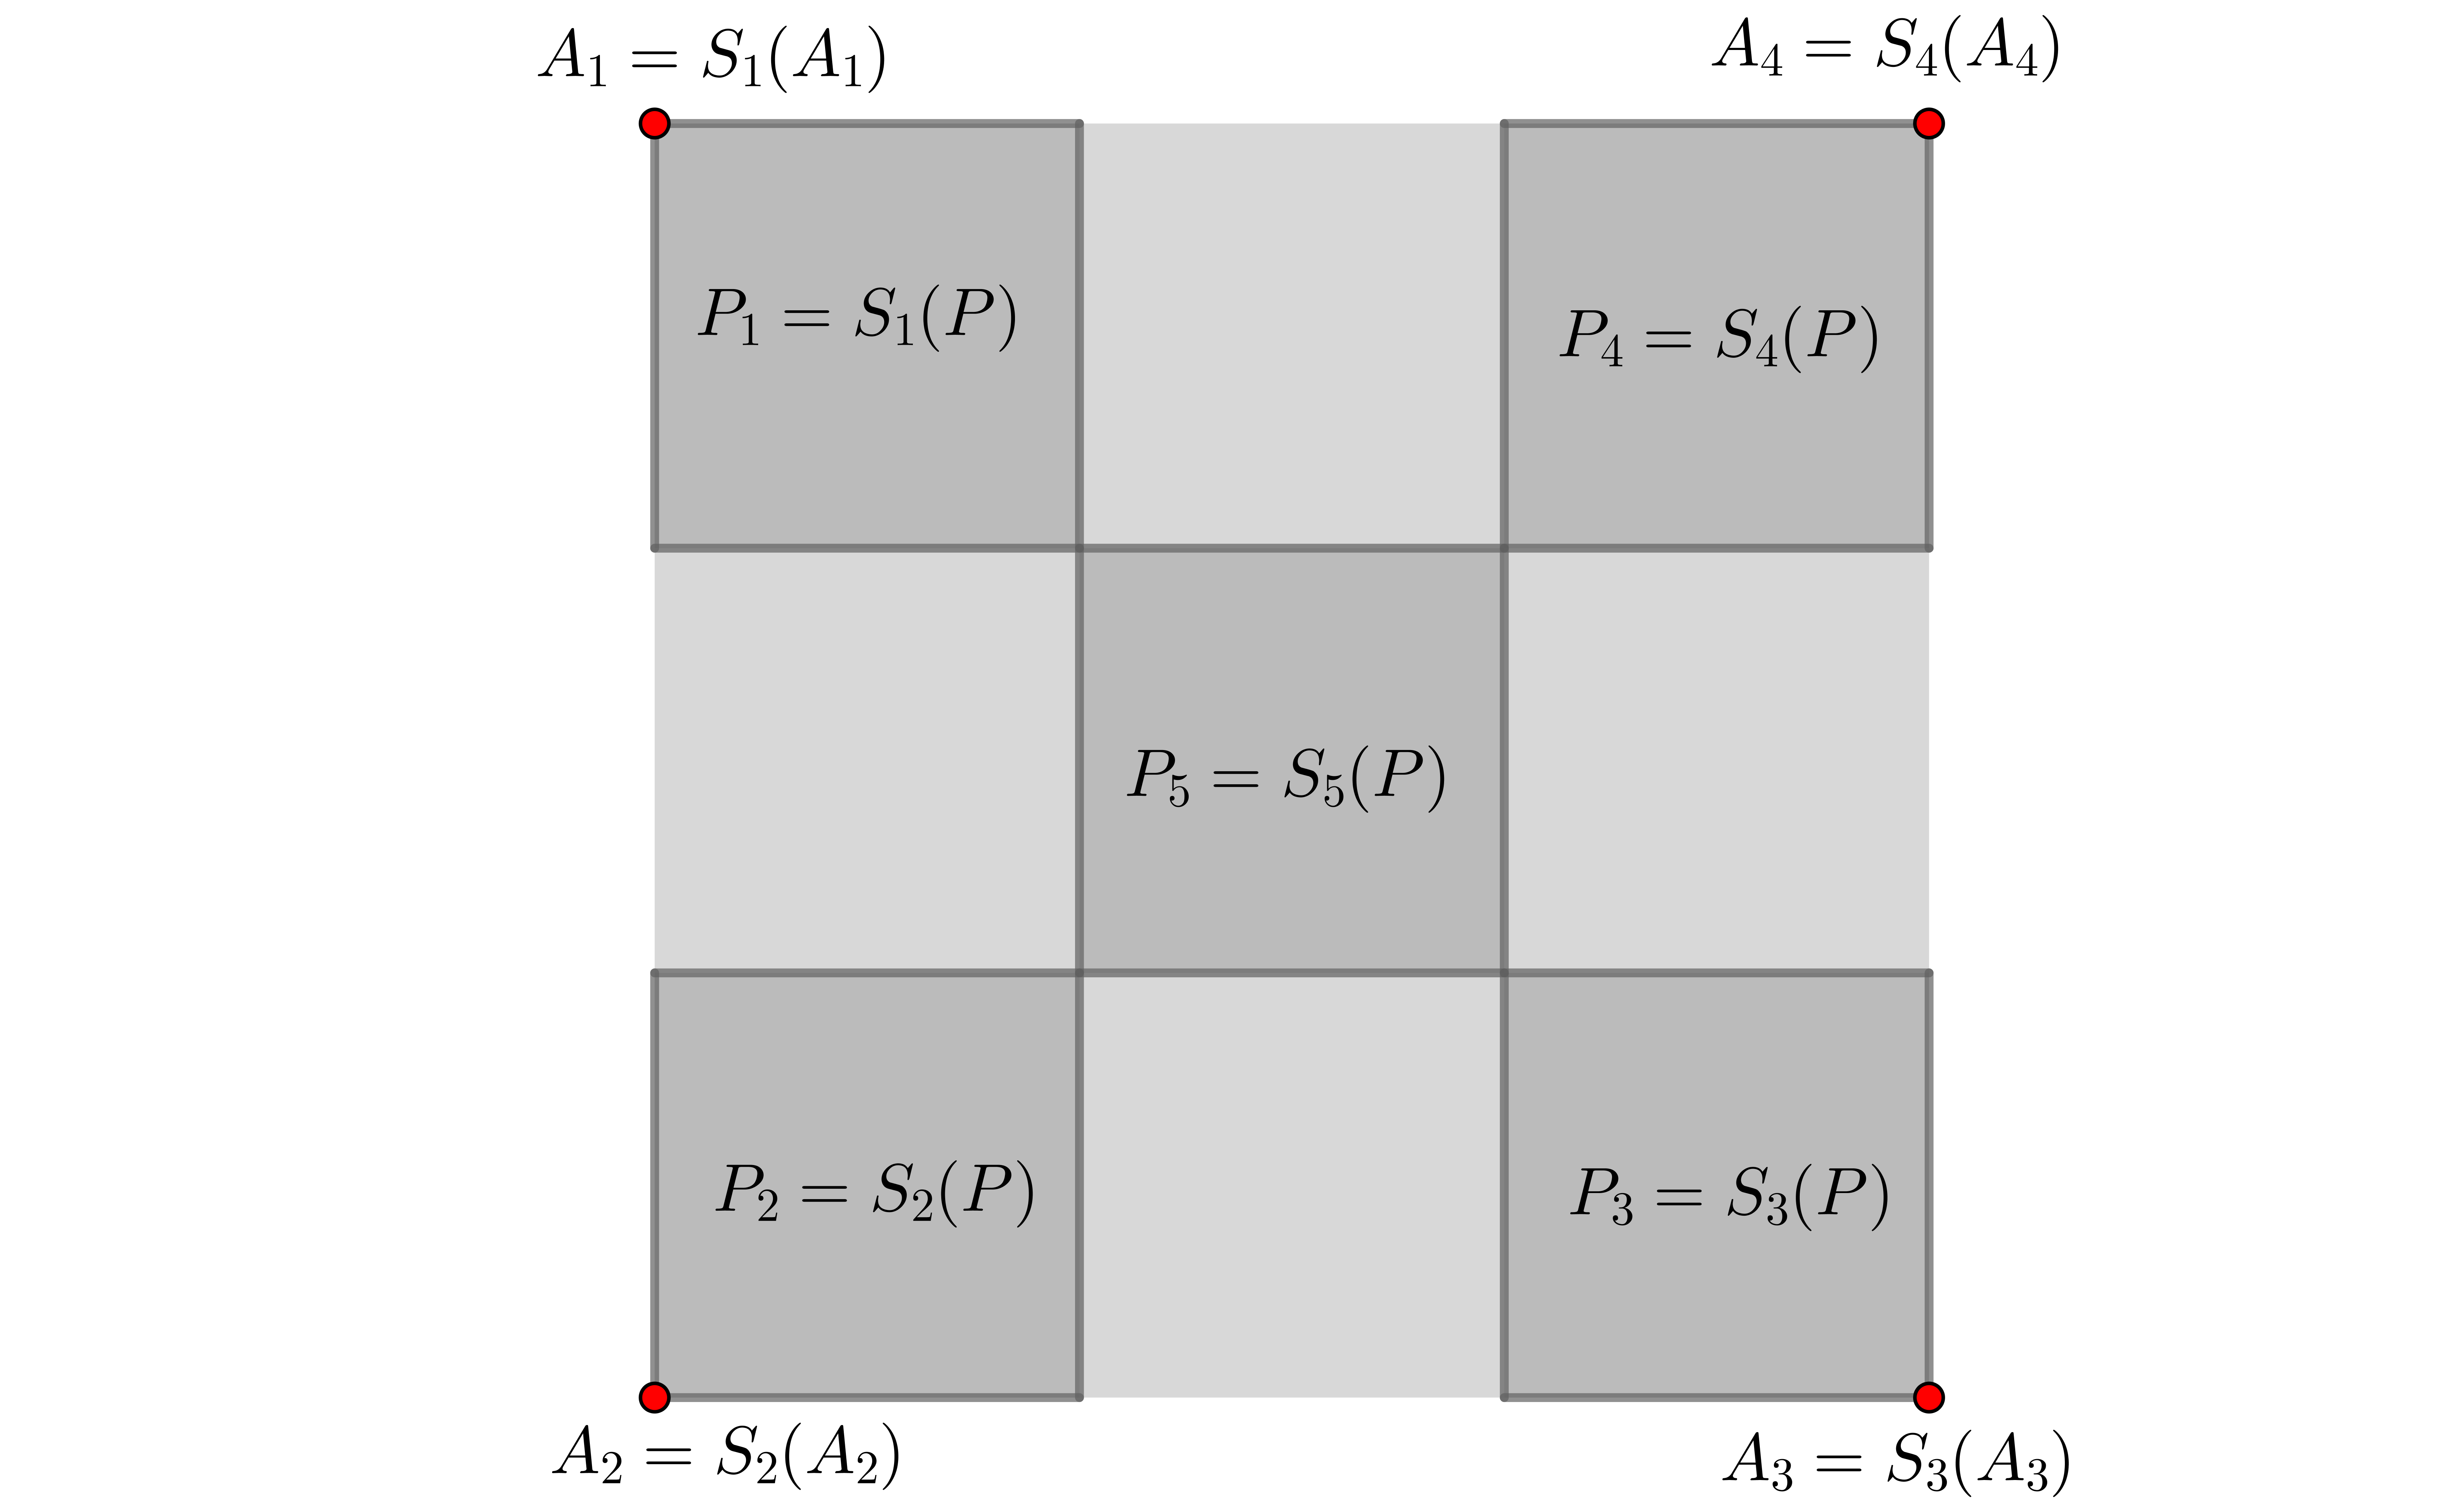
\includegraphics[width=.7\textwidth]{2_24.png}\]}
\only<5>{
{\bf(D1)}  для любого $i\in I$, множество $P_i=S_i(P)\IN P$;\\
{\bf(D2)}  для любых $i\neq j,\ \   i, j \in I,$ $P_i \cap P_j=V_{P_i}\cap V_{P_j}$ ;\\
{\bf(D3)}  $V_P\IN \bigcup\limits_{i\in I}S_i(V_P)$;\\
{\bf(D4)}  множество    ${\wP} = \bigcup \limits_{i = 1}^m P_i$ стягиваемо.
\begin{definition}
Система \ $\eS $, удовлетворяющая условиям {\bf (D1)-(D4)},
называется  стягиваемой $P$-полигональной  системой подобий.
\end{definition}
\begin{theorem} Аттрактор $K$  стягиваемой  $P$-полигональной  системы подобий $\eS$ является дендритом.
\end{theorem}}
\end{frame}


\begin{frame}{Обобщённая полигональная система}

\end{frame}


\begin{frame}{$\delta$-деформация}

\end{frame}


\begin{frame}{}

\end{frame}


\begin{frame}{}

\end{frame}


\begin{frame}{}

\end{frame}


\begin{frame}{}

\end{frame}


\begin{frame}{}

\end{frame}


\begin{frame}{}

\end{frame}


\begin{frame}{}

\end{frame}


\begin{frame}{}

\end{frame}


\begin{frame}{}

\end{frame}


\begin{frame}{}

\end{frame}


\begin{frame}{}

\end{frame}


\begin{frame}{}

\end{frame}


\begin{frame}{}

\end{frame}


\begin{frame}{}

\end{frame}


\begin{frame}{}

\end{frame}


\begin{frame}{}

\end{frame}


\begin{frame}{}

\end{frame}


\begin{frame}{}

\end{frame}


\begin{frame}{}

\end{frame}


\end{document}